%http://cs.pugetsound.edu/~jross/courses/cs240/project/requirements/
%Animation Group
\documentclass[12pt]{article}
\usepackage{graphicx}
\begin{document}

% Front Page
\begin{titlepage}
	\begin{center}
	\huge  Edith \\
	\vspace*{\fill}%
 	\huge \textsc{\textbf{Animation System \\Intermediate Report} }	
	\bigskip 
	\rule{130mm}{.1pt}
	\textsc{\textbf{October 7, 2013 \\ Revised: October 18, 2013} \\ }	
	\vspace*{\fill}%
	Eric Lund \\
	Kramer Canfield \\ 
	Zeke Rosenberg \\
	Calder Whiteley \\
	Jon Youmans
	\end{center}
\end{titlepage}

\section{\emph{Animation System Structure}}%Create a section for the introduction
\subsection{Module Components}
\begin{enumerate}
\item Parser
\begin{enumerate}
\item The Animation System will be receiving instructions for animations in JSON format. This subsystem will take the instructions and actually call the functions with correct inputs. Our required interface is JSON, but more specifically a JSON entry with the following elements:
\item \{``function name" : ``jump(x1, x2, y1, y2)", ``Image Name": ``example.png", ``Audio File Name": ``soundFile.mp3"\}
\item There will be certain instructions that might not have specific pieces of information, such as an animation without an associated sound. In a case where this occurs, input ``null" in the appropriate location.

\end{enumerate}

\item Controller
\begin{enumerate}
\item Once we have parsed JSON inputs into separate instructions, the Controller subsystem will carry out those instructions and send media creation and display instructions to the HTML5 canvas. This component will have several important interactions.
\item The Controller will take the raw data about the media instructions and create a list of instructions to send to the HTML5 canvas for drawing and playing sounds. The instructions for the canvas will be stored in a Scene Array, which will later be useful for play(), pause(), and seek().
\end{enumerate}

\item Scene Array
\begin{enumerate}
\item The Scene Array sub-component of the Controller simply holds a list of frames, each frame being one step of the animation process. These will be stored in an array so that playback control functions (called by another team) will allow the user to select a time to view from, and the Scene Array can then get the necessary media and display it. 
\end{enumerate}
\end{enumerate}



\noindent\subsection{Design Rationale}
The Parser is its own sub-system rather than being part of the Controller because interpreting the input is a one-way process and the Controller does not need to access the raw inputs. The Scene Array component is a sub-component of the Controller to allow for easier access to the media instructions in the array.


\noindent\subsection {Interactions}
\begin{enumerate}
\item The Animation System will have no direct interaction with the ``programmer" because the Animation System is a back-end module and is dependent on other frameworks and modules such as a canvas.
\item The Animation System interacts with the Story Creator module, who feeds us the JSON instructions to be interpreted with the parser and carried out. It also interacts with the visual editor team, which will be providing the images, sounds, etc. to be used following the JSON instructions. Finally, we will be giving our output to the (some other team here) to be painted on the canvas.
\item The only other requirement for the Animation System is that we are using a 3rd party library, ``OCanvas', to make animations easier and better looking. This library works directly with an HTML5 canvas, so there are minimal if any changes from other teams. This can be found at http://ocanvas.org/docs

\end{enumerate}



\subsection{Activity Diagram}
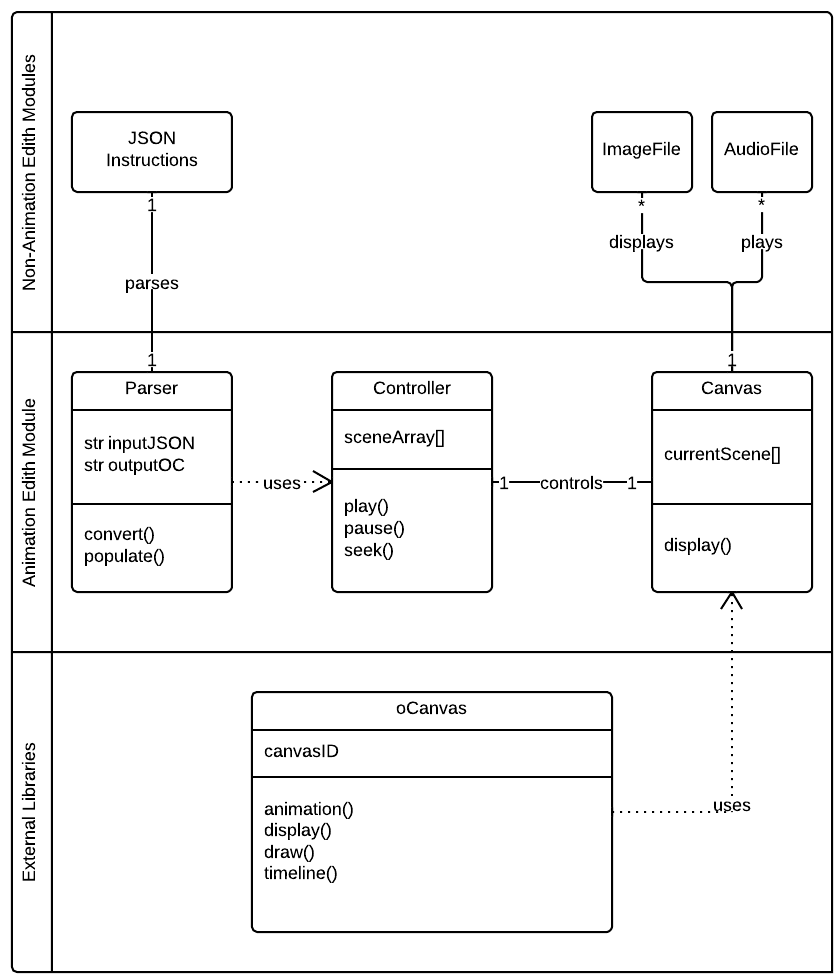
\includegraphics[scale=.45]{AnimationUMLClassDiagram.png}
\\UML Class Diagram
\pagebreak

%Glossary/References
\section{\emph{Project Status}}
\noindent\subsection{Current State of Implementation}

Our team has created an example HTML file which creates a HTML5 canvas with a sprite. This file implements the external HTML library, oCanvas which we use to bind several animations to the sprite. These animations can be invoked on the sprite by pressing the associated buttons. Even though this example simulates a final implementation of a scene, it provides a good example of how the sprite will react to certain animations in which we create. 

The animations we have implemented are rotate 360 degrees, vertical jump, forward jump and a reverse jump. Each animation also has an ease function associated that when applied, effects the playback of the animations to create different effects. For example, our jump animation looks best with a ease-in-out-bounce ease and a rotation looks best with a smoother easing function. Until we get a JSON file from the Story Creator we will continue to add animation elements on our example. 
	
\noindent\subsection{Member Responsibilities}


\begin{description}
  \item[Kramer:] \hfill \\
  Documentation with flexible responsibility between groups. Kramer will help where ever help is needed. Kramer will also be the contact point for other groups.
  \item[Zeke and Jon:] \hfill \\
  JSON parsing
  \item[Eric and Calder:] \hfill \\
  Scene array and controller
\end{description}

\noindent\subsection{Implementation Timeline}
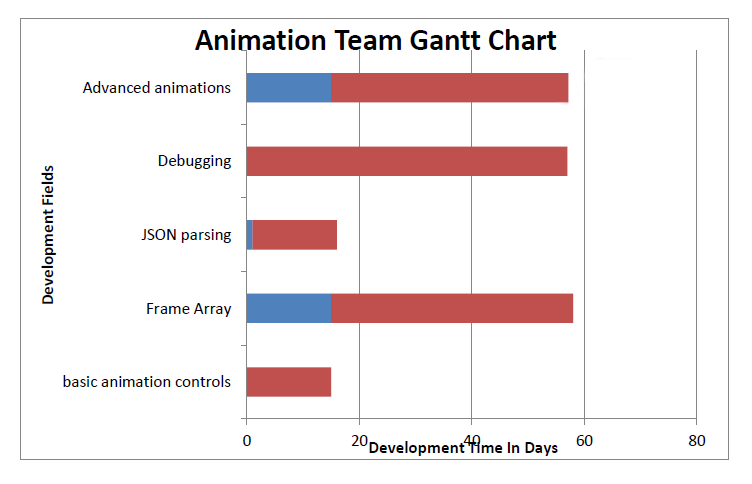
\includegraphics[scale=.45]{AnimationGanttChart.png}
\linebreak
\linebreak
Basic animation controls and the parsing of JSON instruction sets must be handled first in order to allow integration with other modules.  After the basic animations and JSON parsing are implemented the Frame Array will be added to allow playback controls.  The animation set will be expanded alongside the implementation of the Frame Array to provide the programmer with a wider variety of available animations.

\noindent\subsection{Development Reflection}
Scheduling has been difficult due to the members of the Animation Team's varied availability.  This has managed by team members uploading individual schedules to a group Google Calendar which then allows easier meeting planning.  The group has decided to use the oCanvas library to augment the built in canvas tool of HTML5.



%Glossary/References
\section{\emph{Glossary/References}}
Glossary:
\begin{itemize}
	\item Programmer: The individual who is using Edith through his/her web browser to learn how to program.
	\item Sprite: a computer graphic that may be moved on-screen and otherwise manipulated as a single entity (New Oxford American Dictionary (American English))
\end{itemize}
	

	
\end{document}
